\documentclass{article}
\usepackage{lmodern}
\usepackage{amssymb,amsmath}
\usepackage[T1]{fontenc}
\usepackage[utf8]{inputenc}
\usepackage{amsfonts}

% Para el código
\usepackage{listings}
\usepackage{xcolor}
\definecolor{gray}{rgb}{0.5,0.5,0.5}
\newcommand{\n}[1]{{\color{gray}#1}}
\lstset{numbers=left,numberstyle=\tiny\color{gray}}

% Para la tabla
\usepackage{tikz}
\usetikzlibrary{matrix, shapes, decorations, positioning, decorations.pathreplacing}
\tikzstyle{invtable}=[matrix of nodes,inner sep=0pt, nodes in empty cells,
nodes={minimum size=0.8cm,anchor=center,align=center}]
%\tikzstyle{br}=[decoration={brace,amplitude=0.5em},decorate, thick]
\everymath{\displaystyle}

% Entorno para estilo de ejercicios
\newenvironment{ejercicio}[1]
{\noindent\textbf{#1} \vspace*{5mm}}{\vspace*{5mm}}

% Comando para destacar el resultado
\newcommand{\resultado}[1]{\colorbox{gray!10}{$\displaystyle#1$}}


\begin{document}
%\include{ej1}
\begin{ejercicio}
{2. Determinar la eficiencia de la siguiente función:}
\begin{lstlisting}[
language=C++, directivestyle={\color{black}},
emph={int,char,double,float,unsigned}]
int cualeslaeficiencia(bool existe)
{
  int sum2=0; int k,j,n;
  if(existe)
    for(k=1; k<=n; k*=2)
      for(j=1; j<=k; j++)
        sum2++;
  else
    for(k=1; k<=n; k*=2)
      for(j=1; j<=n; j++)
        sum2++;
  return sum2;
}
\end{lstlisting}
\vspace*{5mm}

Primero analizamos los dos bucles del condicional:

\begin{itemize}

\item El \textbf{primer bucle} (\n{5-7}) se repite $\log_2(n) + 1$ veces,
ya que $k$ se  multiplica por 2 cada vez.
El bucle interior (\n{6-7}) repite una sentencia $O(1)$ $k$ veces.
Cada $k$ puede escribirse de la forma $2^i$ para $i \in \mathbb{N}$.
Es decir, el número de pasos del bucle será:

\[\sum_{i=0}^{\log_2(n)+1} 2^i = 2^{\log_2{n}+1} -1 = 2n -1 \in O(n)\]

\item El \textbf{segundo bucle} (\n{9-11}) se repite $\log_2(n) +1$ veces.
El bucle interior (\n{10-11}) repite una sentencia $O(1)$ $n$ veces.
Es decir, el número de pasos del bucle será, por la regla del producto:
$O(n\log(n))$
\end{itemize}

Podríamos considerar sólo el segundo bucle, dado que el número
de sentencias ejecutadas en el primero es estrictamente menor
que en el segundo.
Como estamos ante un condicional tomamos el máximo de ambas
partes, obteniendo que la eficiencia es:

\[O(1) + O(\max\{n,n\log n\}) + O(1)  = \resultado{O(n\log n)}\]

\end{ejercicio}

\pagebreak
%\begin{ejercicio}{
3. Ordenar la siguiente lista de acuerdo a la notación $O$}

Utilizaremos las siguientes propiedades:
\begin{enumerate}
  \item $f(n) \leq g(n) \implies 2^{f(n)} \leq 2^{g(n)}$.
  ($n_0' = n_0$ y $c'= 2^c$)
  \item $0 < a_1 < a_2 \implies n^{a_1} \leq n^{a_2}$.
  ($n_0 = c = 1$)
\end{enumerate}

\vspace*{10mm}

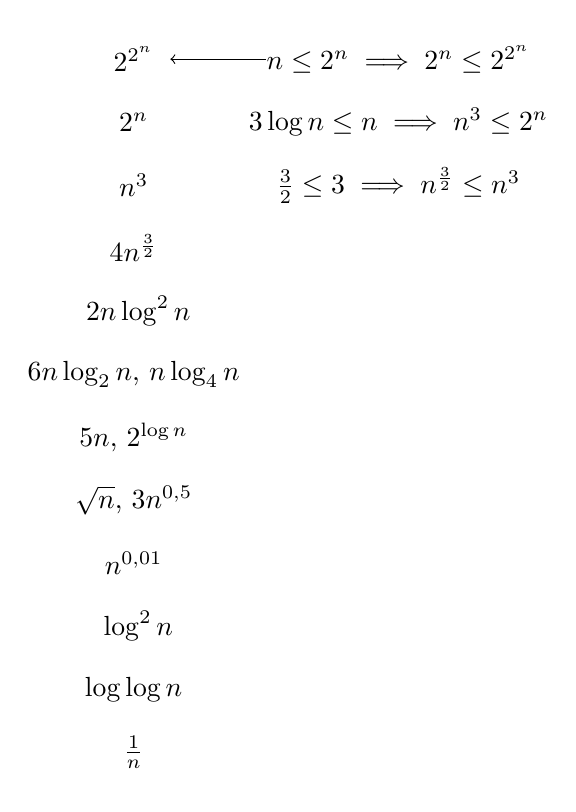
\begin{tikzpicture}
\node[invtable] (m) {
  $2^{2^n}$ & $n \leq 2^n \implies 2^n \leq 2^{2^n}$\\
  $2^{n}$ & $3\log n \leq n \implies n^3 \leq 2^n$\\
  $n^3$ & $\frac{3}{2} \leq 3 \implies n^{\frac{3}{2}} \leq n^3$\\
  $4n^{\frac{3}{2}}$ & \\
  $2 n \log^2 n$& \\
  $6n \log_2 n$, $n \log_4 n$ & \\
  $5n$, $2^{\log n}$ & \\
  $\sqrt{n}$, $3n^{0,5}$ & \\
  $n^{0,01}$ & \\
  $\log^2 n$& \\
  $\log \log n$ & \\
  $\frac{1}{n}$ & \\
};

\draw[->] (m-1-2) -- (m-1-1);
\end{tikzpicture}
\end{ejercicio}

%\begin{ejercicio}
{4. Para cada función $f(n)$ y cada tiempo $t$ de la tabla siguiente, determinar el mayor tamaño de un problema que puede ser resuelto en un tiempo $t$ (suponiendo que el algoritmo para resolver el problema tarda $f(n)$ microsegundos, es decir, $f(n) \times 10^{-6}$ sg.)}

\begin{itemize}
\item Los valores de la fila $f(n) = \log_2 n$ deben ser los máximos que, siendo $s$ el tiempo en segundos:
$$
\log_2 n \times 10^{-6} \le s \implies \log_2 n \le s \times 10^6 \implies n \le 2^{s \times 10^6}
$$

Sustituyendo $s$ por el tiempo de cada columna obtendríamos los resultados, con $2$ como base. Sin embargo, dado que en la tabla aparece un resultado usando $10$ como base, haremos lo mismo:
$$
n \le 2^{s \times 10^6} \implies \log_{10} n \le \log_{10} 2^{s \times 10^6} \implies \log_{10} n \le {s \times 10^6} \times \log_{10} 2 \implies n \le 10^{{s \times 10^6} \times \log_{10} 2}
$$

La última expresión nos permite obtener los valores máximos posibles de $n$ usando una potencia de $10$. Sustituyendo $s$ en cada columna por el valor correspondiente y redondeando a la baja, obtendremos los elementos de la fila. Dado que los números son muy grandes, daremos una expresión aproximada.

\item Los valores de la fila $f(n) = n$ cumplen que $
n \times 10^{-6} \le s$, es decir, $n \le s \times 10^6$. Los números siguen siendo muy grandes como para no aproximarlos, así que algunos estarán aproximados.

\item Los valores de la fila $f(n) = n\ \log_2 n$ serán obtenidos hallando la solución de $h(n) = 0$, siendo $h(n) = n\ \log_2(n) - s \times 10^6$.

Invertir $h(x)$ resulta incómodo, por ello aprovecharemos que $h(n)$ es una función continua, que $h(n) < 0 \ \ \forall s \ge 1$ y que $\displaystyle \lim_{n \to +\infty} h(n) = +\infty \ \ \forall s \ge 1$. Por tener esas propiedades, el teorema de Bolzano determina que, para algún valor de abscisa positivo (no necesariamente entero) de $n$, la función devolverá $0$.

Usaremos un software que permite aproximar con precisión arbitraria el valor en el que una función continua se anula: Maxima y la función \texttt{find\_root} con los parámetros $n\ \log_2(n) - s \times 10^6, n, 1, 10^{30}$ para obtener los valores.

\item Los valores de la fila $f(n) = n^3$ serán tales que $n^3 \times 10^{-6} \le s$ y, por consiguiente, $n \le \sqrt[3] {s \times 10^6}$. Esta vez los números empiezan a ser manejables en una tabla tan pequeña, por lo que hallaremos el valor que cumple la igualdad y redondearemos el valor a la baja para obtener el resultado exacto pedido.

\item Los valores de la fila $f(n) = 2^n$ son los máximos posibles que cumplen $2^n \times 10^{-6} \le s$ y, por consiguiente, $n \le \log_2 (s \times 10^6)$ y $n \le 6\log_2 10 + \log_2 s$. Hallaremos el valor que cumple la igualdad y lo truncaremos.

\item Los valores de la fila $f(n) = n!$ serán aquellos tales que $n! \times 10^{-6} \le s$. Ello lleva a que $n! \le s \times 10^6$. $n!$ crece tan rápido que es viable hallar los valores correctos probando todos los $n$ a partir de 1 hasta encontrar el primero que incumpla la igualdad, y tomar el inmediatamente anterior.

\end{itemize}

Aplicando lo descrito arriba, la tabla obtenida resulta ser la siguiente (se ha considerado la longitud de 1 año como exactamente 365 días):

\vspace*{0.3cm}

\bgroup
\def\arraystretch{1.6}
\setlength\tabcolsep{12.5px}
\begin{tabular}{|c|c|c|c|c|c|}
	\hline
	\multirow{2}{*}{$f(n)$} & \multicolumn{5}{|c|}{$t$}\\
	\cline{2-6}
	& 1 sg. & 1 h. & 1 semana & 1 año & 1000 años \\
	\hline
	$\log_2 n$ & $\approx 10^{301030}$ & $\approx 10^{10^9}$ & $\approx 10^{1,8 \times 10^{11}}$ & $\approx 10^{9,5 \times 10^{12}}$ & $\approx 10^{9,5 \times 10^{15}}$  \\
	\hline
	$n$ & $10^6$ & $3,6 \times 10^9$ & $\approx 6 \times 10^{11}$ & $\approx 3,15 \times 10^{13}$ & $\approx 3,15 \times 10^{16}$ \\
	\hline
	$n \log_2 n$ & $62746$ & $\approx 1,33 \times 10^8$ & $\approx 1,78 \times 10^{10}$ & $\approx 7,98 \times 10^{11}$ & $\approx 6,41 \times 10^{14}$ \\
	\hline
	$n^3$ & $100$ & $1532$ & $8456$ & $31593$ & $315938$ \\
	\hline
	$2^n$ & $19$ & $31$ & $39$ & $44$ & $54$ \\
	\hline
	$n!$ & $9$ & $12$ & $14$ & $16$ & $18$ \\
	\hline
\end{tabular}
\egroup
\end{ejercicio}

\end{document}
